%%%%%%%%%%%%%%%%%%%%%%%%%%%%%%%%%%%%%%%%%%%%%%%%%%%%%%%%%%%%%%%%%%%%%%
% Lớp 10 | Véctơ (chưa xét tọa độ) | Khái niệm véctơ
% Dạng 0H5?1-2: Xét phương và hướng của các véctơ
% Số câu: 3  (sinh tự động bởi tach_cau.py; từ nay thầy sửa trực tiếp file này)
%%%%%%%%%%%%%%%%%%%%%%%%%%%%%%%%%%%%%%%%%%%%%%%%%%%%%%%%%%%%%%%%%%%%%%

%%%%%%%%%%%%%%%% TRẮC NGHIỆM 4 PHƯƠNG ÁN %%%%%%%%%%%%%%%%

% nguồn: MaHoaNH_TracNghiem_Lop10
\begin{ex}%[0H5N1-2]%[ma:c69ae3fa]
	Mệnh  đề nào dưới đây đúng?
	 \choice
		{\True Hai vectơ cùng phương với một vectơ thứ ba khác $\overrightarrow{0}$  thì cùng phương}
		{Hai vectơ ngược hướng với một vectơ thứ ba  thì cùng hướng}
		{Hai vectơ cùng phương với một vectơ thứ ba  thì cùng phương}
		{Hai vectơ cùng phương với một  vectơ thứ ba thì cùng hướng}
	 \loigiai{
		Hai vectơ cùng phương với một vectơ thứ ba khác  $\overrightarrow{0}$ thì cùng phương.
	 }
\end{ex}

% nguồn: MaHoaNH_TracNghiem_Lop10
\begin{ex}%[0H5N1-2]%[ma:9d31db7e]
	Cho  $3$ điểm $M$, $N$, $P$ thẳng hàng thoả mãn $N$ nằm giữa $M$ và $P$. Khi đó cặp vectơ nào sau đây cùng hướng?
	\choice 
		{\True $\overrightarrow{MN}$ và $\overrightarrow{MP}$} 
		{$\overrightarrow{MN}$ và $\overrightarrow{PN}$} 
		 {$\overrightarrow{NM}$ và $\overrightarrow{NP}$}
		 {$\overrightarrow{MP}$ và $\overrightarrow{PN}$}
	 \loigiai{
		\begin{center}
			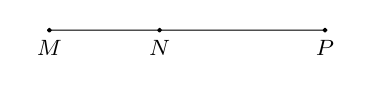
\begin{tikzpicture}[scale=0.7,line join=round,line cap=round,font=\footnotesize,>=stealth]
					\draw[fill =  black] (0,0) circle (1pt) node[below]{$M$}
						-- (2,0) circle (1pt)  node[below]{$N$}
						--  (5,0) circle (1pt) node[below]{$P$};
				\end{tikzpicture}
		\end{center}
		Nhìn vào hình vẽ  ta thấy cặp vectơ cùng hướng là $\overrightarrow{MN}$ và $\overrightarrow{MP}$.
	 }
\end{ex}


%%%%%%%%%%%%%%%% ĐÚNG/SAI %%%%%%%%%%%%%%%%

% nguồn: MaHoaNH_DungSai_Lop10
\begin{ex}%[0H5H1-2]%[ma:0be35690]
	Cho tam giác  $ABC$ có $M$, $N$, $P$ lần lượt là trung điểm $BC$, $CA$, $AB$.
	\choiceTF 
		 {\True $\overrightarrow{AB}$ và $\overrightarrow{MN}$ cùng phương}
		{Số vectơ khác vectơ-không, cùng phương  với $\overrightarrow{AB}$ (không tính $\overrightarrow{AB}$) có điểm đầu, điểm cuối lấy từ các điểm đã cho là $6$}
		{$\overrightarrow{AP}$  và $\overrightarrow{PB}$ ngược hướng}
		{\True Số vectơ khác vectơ-không, cùng hướng với $\overrightarrow{BC}$ (không tính $\overrightarrow{BC}$) có  điểm đầu, điểm cuối lấy từ các điểm đã cho là $3$}
	\loigiai{ 
	 \immini
		 {
		Ta có 
		\begin{itemchoice}
			\itemch  Vì $MN\parallel AB$.
			\itemch Vì có $7$ vectơ khác vectơ-không, cùng phương với $\overrightarrow{AB}$ (không tính $\overrightarrow{AB}$) có điểm  đầu, điểm cuối lấy từ các điểm đã cho, cụ thể là $\overrightarrow{AP}$, $\overrightarrow{PA}$, $\overrightarrow{BA}$, $\overrightarrow{BP}$, $\overrightarrow{PB}$, $\overrightarrow{NM}$, $\overrightarrow{MN}$.
			\itemch Vì $\overrightarrow{AP}$  và $\overrightarrow{PB}$ cùng hướng.
			\itemch Vì có $3$ vectơ khác vectơ-không, cùng hướng với $\overrightarrow{BC}$ (không tính $\overrightarrow{BC}$) có điểm đầu, điểm cuối lấy từ các điểm đã cho, cụ  thể là $\overrightarrow{BM}$, $\overrightarrow{MC}$, $\overrightarrow{PN}$.
		\end{itemchoice}
		 }
		 {
		\begin{tikzpicture}[line join=round,line cap = round,>=stealth,scale=.7,font=\footnotesize,transform shape]
				\foreach \x/\y/\z/\g  in
					{ 
					0/0/B/-135,2/4/A/90,6/0/C/-45,1/2/P/135,4/2/N/60,3/0/M/-90 
				} 
				\draw[fill=black] (\x,\y) circle (1pt) coordinate  (\z)
					($(\z)+(\g:3.5mm)$)  node{$\z$};
				 \draw (A)--(C);
				\draw[->] (A)--(B); 
				 \draw[->] (M)--(N);
				\draw[->]  (A)--(P);
				 \draw[->] (P)--(B);
				\draw[->]  (B)--(C);
			\end{tikzpicture}
		 }
	} 
\end{ex}
